\documentclass[a4paper]{article}     
\usepackage{amsfonts}
\usepackage{amsmath}
\usepackage{amssymb}
\usepackage{graphicx}
\usepackage{cancel}

\newcommand{\asa}{\Leftrightarrow} %als slechts als
\newcommand{\adR}{\Rightarrow} %als dan Rechts
\newcommand{\adL}{\Leftarrow}
\newcommand{\Lh}{\left(} %Links haakje
\newcommand{\Rh}{\right)}
\newcommand{\Lv}{\left[} %Links vierkanthaakje
\newcommand{\Rv}{\right]}
\newcommand{\La}{\left\{} %Links acolade
\newcommand{\Ra}{\right\}}
\newcommand{\Ras}{\right.} %Rechts acolade stelsel (omdat om stelsels te maken heb je een punt nodig
\newcommand{\pnR}{\rightarrow} %pijl naar Rechts
\newcommand{\limiet}{\lim\limits_}
\newcommand{\schrap}{\cancel}
\newcommand{\schrapb}{\bcancel} %backslash
\newcommand{\schrapk}{\xcancel} %kruis
\newcommand{\vervang}{\cancelto}
\newcommand{\stijg}{\nearrow} %stelt stijgende pijl voor
\newcommand{\daal}{\searrow} %stelt dalende pijl voor

\begin{document}

\noindent \large Auteur: Yoren Collier \\
\noindent \large Studierichting: Informatica\\
\noindent \large Oefeningenreeks 3G nr. 18.1\\

\medskip

\normalsize

$f(x) = x\sqrt{x}$\\

dom, Im, periode, snijpunten assen\\

$\operatorname{dom} f = \mathbb{R}^+, \operatorname{Im} f = \mathbb{R}^+, \operatorname{per.} f = / $\\

$0 = x\sqrt{x} \asa x = 0$ of $\sqrt{x} = 0$\\

Snijpunt(en) x-as: $\Lh  0, 0 \Rh$ , Snijpunt $Y$-as: $\Lh 0, 0 \Rh$\\

Asymptoten:\\

VA: Geen VA mogelijk\\

Ha: $\limiet{x \pnR +\infty} f(x) = \limiet{x \pnR +\infty} x = +\infty \adR$ Geen HA\\

$\limiet{x \pnR -\infty} f(x) =$ bestaat niet\\

SA: $\limiet{x \pnR +\infty} \dfrac{f(x)}{x} = \limiet{x \pnR +\infty} \dfrac{\schrap{x}\sqrt{x}}{\schrap{x}} = +\infty \adR$ Geen SA\\

Afgeleiden:\\

$\dfrac{df}{dx}(x) = x \cdot \dfrac{1}{2\sqrt{x}} + \sqrt{x} = \dfrac{x}{2\sqrt{x}} + \dfrac{2x}{2\sqrt{x}} = \dfrac{3\schrap{x} \sqrt{x}}{2\schrap{x}} = \dfrac{3\sqrt{x}}{2} $\\

$\dfrac{d^2f}{dx^2}(x) = \dfrac{3}{2} \cdot \dfrac{1}{2\sqrt{x}} = \dfrac{3}{4\sqrt{x}}$\\

\begin{tabular}{c|c|c|cc}
     $x$&  $-\infty$  &  $0$         &            &  $+\infty$  \\ \hline
 $f'(x)$&  $///$      &  $0$         &  $+$       &  $+$   \\ \hline
$f''(x)$&  $///$      &  $|$         &  $+$       &  $+$  \\ \hline
  $f(x)$&  $///$      &  $0$         &  $+$       &  $+$  \\
        &             &  $m(0)$  		 &  $\stijg$  &  $\stijg$  \\
        &             &              &  $\smile$  &  $\smile$  \\
\end{tabular}

\begin{figure}[h]
\centering
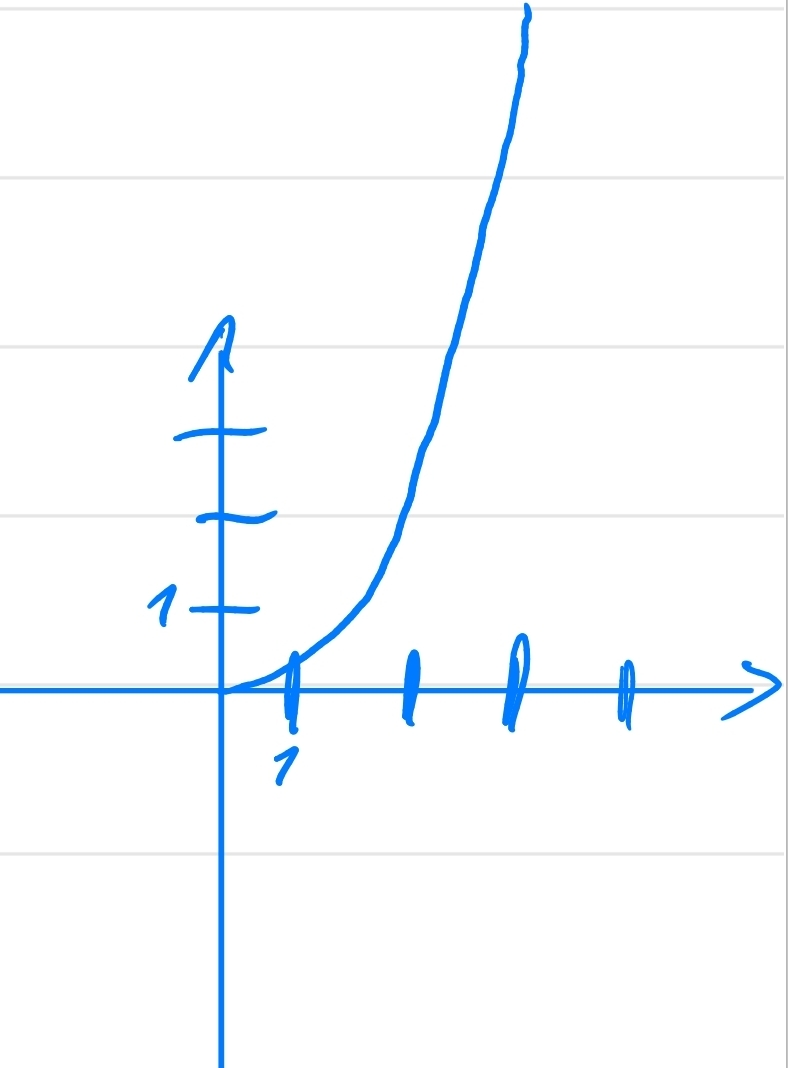
\includegraphics[width=10cm]{./3G-18.1-yoren.collier.INF.jpg}
\end{figure}

\begin{thebibliography}{999}
%\bibitem{a} Referentie
\end{thebibliography}
\end{document} 